\section{Creature Generation}

\subsection{Automatisches Rigging}
Um die Bone-Struktur des generierten Skelettes mit dem Mesh zu verknüpfen, muss bei der 3D-Modellierung der Prozess des Riggings durchlaufen werden. Dieser beschreibt wie sich jeder einzelne Vertex des Meshes mit den Bones in der Szene bewegt. Jeder Vertex kann an beliebig vielen Bones angehängt werden. Durch eine Gewichtung wird bestimmt wie sehr ein Vertex durch der Transformation eines Bones mitbewegt wird.
Da sowohl das Skelett, als auch das gesamte Mesh prozedural generiert werden, kann das Rigging nicht wie üblich in einem Modellierungs-Tool wie Blender~\cite{blender} manuell durchgeführt werden, sondern muss zur Laufzeit des Spiels während der Generierung der Kreaturen geschehen.

Für ein erfolgreiches Rigging ist es wichtig, dass das Skelett bereits sinnvoll in dem Mesh eingebettet ist. Da hier das Mesh aus Metaballs generiert wird, welche um die Bones plaziert sind, können wir hier davon ausgehen, dass das Mesh das Skelett bereits \emph{sinnvoll} umhüllt.

\begin{figure}[h!]
	\centering
	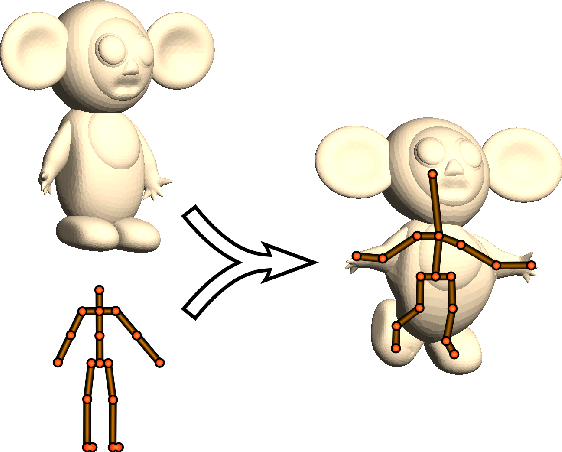
\includegraphics[width=0.7\linewidth]{resources/img/skeleton_embedding.png}
	\caption{Beispiel für ein korrekt eingebettetes Skelett in einem Mesh~\cite{bone_heat_paper}.}
	\label{fig:skeleton_embedding}
\end{figure}

Während der Entwickelung wurde zunächst eine triviale Methode als Zwischenlösung verwendet. Dabei wurden alle Vertices nur an den Bone mit der geringsten Distanz angehängt. Diese Methode ist jedoch visuell unbrauchbar, da bei Bewegung des Skeletts an den Gelenken zwischen den Bones Löcher und verschiedene andere Artefakte entstehen. Es wird also eine Lösung benötigt, die es ermöglicht Vertices an mehrere Bones anzuhängen und die Gewichte so bestimmt, dass das Mesh an den Übergängen zwischen den Bones möglichst natürlich deformiert wird.

Ein bereits bekannter Algorithmus zur automatisch Gewichtsberechnung und Verknüpfung des Meshes ist die Bone-Heat Methode~\cite{bone_heat_paper}. Dieser berücksichtig mehrere zusätzliche Eigenschaften für die Gewichte. Zuerst sollen die Gewichte unabhängig von der Auflösung des Meshes sein. Außerdem müssen die Gewichte sich sanft über den Verlauf der Oberfläche verändern. Die Breite des Übergangs zwischen zwei Bones sollte ungefähr proportional zu der Distanz des Gelenks zur Oberfläche des Meshes sein.....

\begin{figure}[h!]
	\centering
	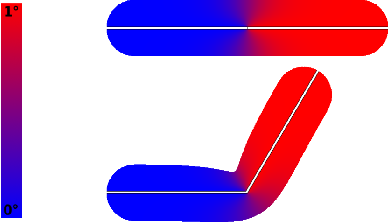
\includegraphics[width=0.7\linewidth]{resources/img/bone_heat_equilibrium.png}
	\caption{Heat equilibrium für zwei Bones~\cite{bone_heat_paper}.}
	\label{fig:bone_heat_equilibrium}
\end{figure}